\chapter{ART OAT File}
\label{chapter:art_oat_file_inspection}

A core element of the recently introduced ART is the file that
gets created by ``dex2oat'' during the installation time of an app,
described in \autoref{section:app_installation}.
Since ART does use AOT compilation, the file format is expected
to be a native code container or something similar. A lot of copy
protection mechanisms are based on the use of native code because
it is supposed to be more secure from reverse code engineering
(which is an assumption so far)
Therefore it's worth to have closer look at that file format
especially since Google does not provide any further information
about it's content and it might have the potential of
revolutionizing the available copy protection mechanisms for
Android or having at least a great impact on them.

By applying the Unix command ``file'' (which can classify
files to MIME-types) to an oat file it comes apparent that
it's actually an ELF file (32 or 64 bit).

\section{ELF File Format}
ELF originally was originally specified by UNIX System Laboratories
(USL) and later by Tool Interface Standards (TIS) and is a common
standard for executables, object code and shared libraries.
It's a quite flexible format for different CPUs and architectures
and does serve as a container for different executable binary
formats.

\begin{figure}[htb]
  \centering
  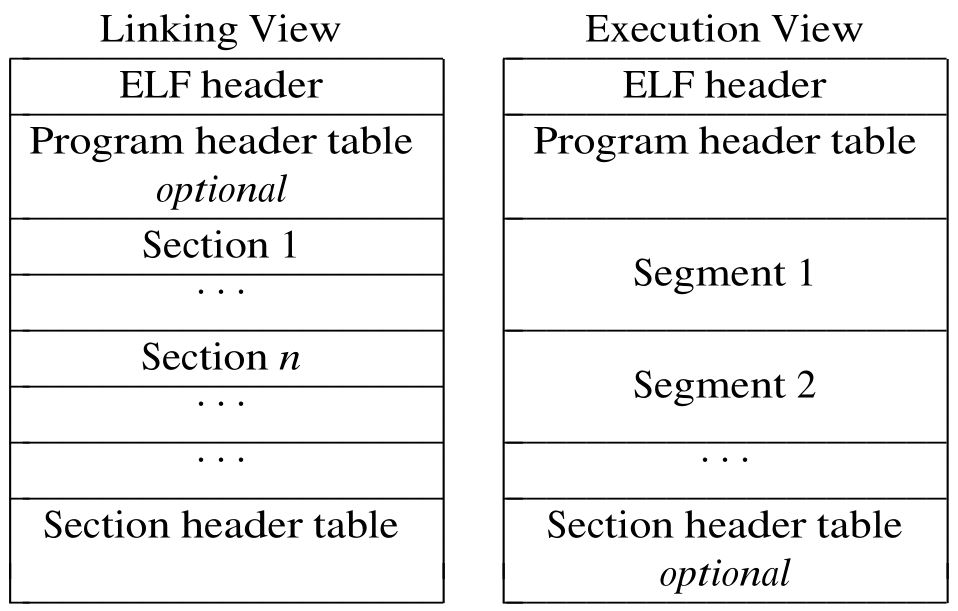
\includegraphics[scale=0.3]{figures/elf_format}
  \caption[ELF file format]{ELF file format}
  \label{fig:elf_format}
\end{figure}

The \autoref{fig:elf_format} shows the basic structure.
Meta data about the file can be read out of the ``ELF header''
section that starts at adress \code{0x00} and does contain
information about the version, file type, target machine and
offsets to program header table and section header table
sections as well as their sizes.
In ART, the file is marked as an shared object with LSB encoding.


\section{OAT File}

\section{DEX File}
